% Generated by Sphinx.
\def\sphinxdocclass[english]{xmosmodern}
\documentclass[  document]{xmosmodern}
\usepackage[utf8]{inputenc}
\DeclareUnicodeCharacter{00A0}{\nobreakspace}

\usepackage{longtable}



\title{Display Spectrum from ADC Quickstart Guide}
\date{November 12, 2013}
\author{}
\newcommand{\sphinxlogo}{}
\newcommand{\releasename}{Release}
\usepackage{xsphinx}
\usepackage{threeparttable}
\usepackage{fancyvrb}
\usepackage{indent}
\renewcommand\bfcode\textbf
\renewcommand\bf\textbf
\graphicspath{{./}{./images/}}
\makeindex

\newcommand\PYGZat{@}
\newcommand\PYGZlb{[}
\newcommand\PYGZrb{]}

\setlength{\emergencystretch}{8em}
\start

\maketitle
\pretoc
\phantomsection\label{quickstart::doc}

%last summary
\begin{inthisdocument}
\item \nameref{quickstart:display-spectrum-from-adc-quickstart}
\item \nameref{quickstart:import-and-build-the-application}
\item \nameref{quickstart:run-the-application}
\item \nameref{quickstart:next-steps}
\end{inthisdocument}


% NON-FULLWIDTH SECTION


In this demonstration we use the following hardware and software:
\begin{itemize}
\item   XP-SKC-U16 sliceKIT

\item   XA-SK-SCR480 Slice Card,

\item   XA-SK-SDRAM Slice Card,

\item   XA-SK-MIXED SIGNAL Slice Card,

\item   module\_level\_meter,

\item   module\_fft\_simple,

\item   module\_display\_controller,

\item   module\_sdram,

\item   module\_lcd,

\item   module\_usb\_tile\_support,

\item   module\_logging,

\item   module\_xassert,

\end{itemize}



together to create a level-meter kind of spectral display on an LCD for an analog audio input. This application showcases the use of multichannel ADC in an xCORE-USB series XMOS device to sample the analog input, and real-time rendering and display of spectrum by taking short-time fourier transform.



% NON-FULLWIDTH SECTION
\section{Hardware Setup}
\label{quickstart:display-spectrum-from-adc-quickstart}\label{quickstart:display-spectrum-from-adc-quickstart-guide}\label{quickstart:hardware-setup}

The XP-SKC-U16 sliceKIT Core board has four slots with edge connectors: \verb`DIAMOND`, \verb`SQUARE`, \verb`A` and \verb`U`.


To setup up the system:
\begin{enumerate}
\item   Connect XA-SK-SDRAM Slice Card to the XP-SKC-U16 sliceKIT Core board using the connector marked with \verb`SQUARE`.

\item   Connect XA-SK-SCR480 Slice Card with LCD to the XP-SKC-U16 sliceKIT Core board using the connector marked with \verb`DIAMOND`.

\item   Connect XA-SK-MIXED SIGNAL Slice Card to the XP-SKC-U16 sliceKIT Core board using the connector marked with \verb`A`.

\item   Give the two channels of audio input from a PC or a mobile to pins 1 and 2 of J2 on the mixed signal slice card using a suitable cable. The ground is connected to pin 4 of J3.

\item   Connect the xTAG-2 to sliceKIT Core board.

\item   Connect the xTAG-2 to host PC. Note that the USB cable is not provided with the sliceKIT starter kit.

\item   Set the \verb`xCONNECT LINK` to \verb`OFF` on the sliceKIT Core board.

\item   Ensure the jumper on the XA-SK-SCR480 is bridged if the back light is required.

\item   Switch on the power supply to the sliceKIT Core board.

\end{enumerate}

\begin{figure}[h]
\begin{sidecaption}{Hardware Setup for Display Spectrum from ADC Demo}

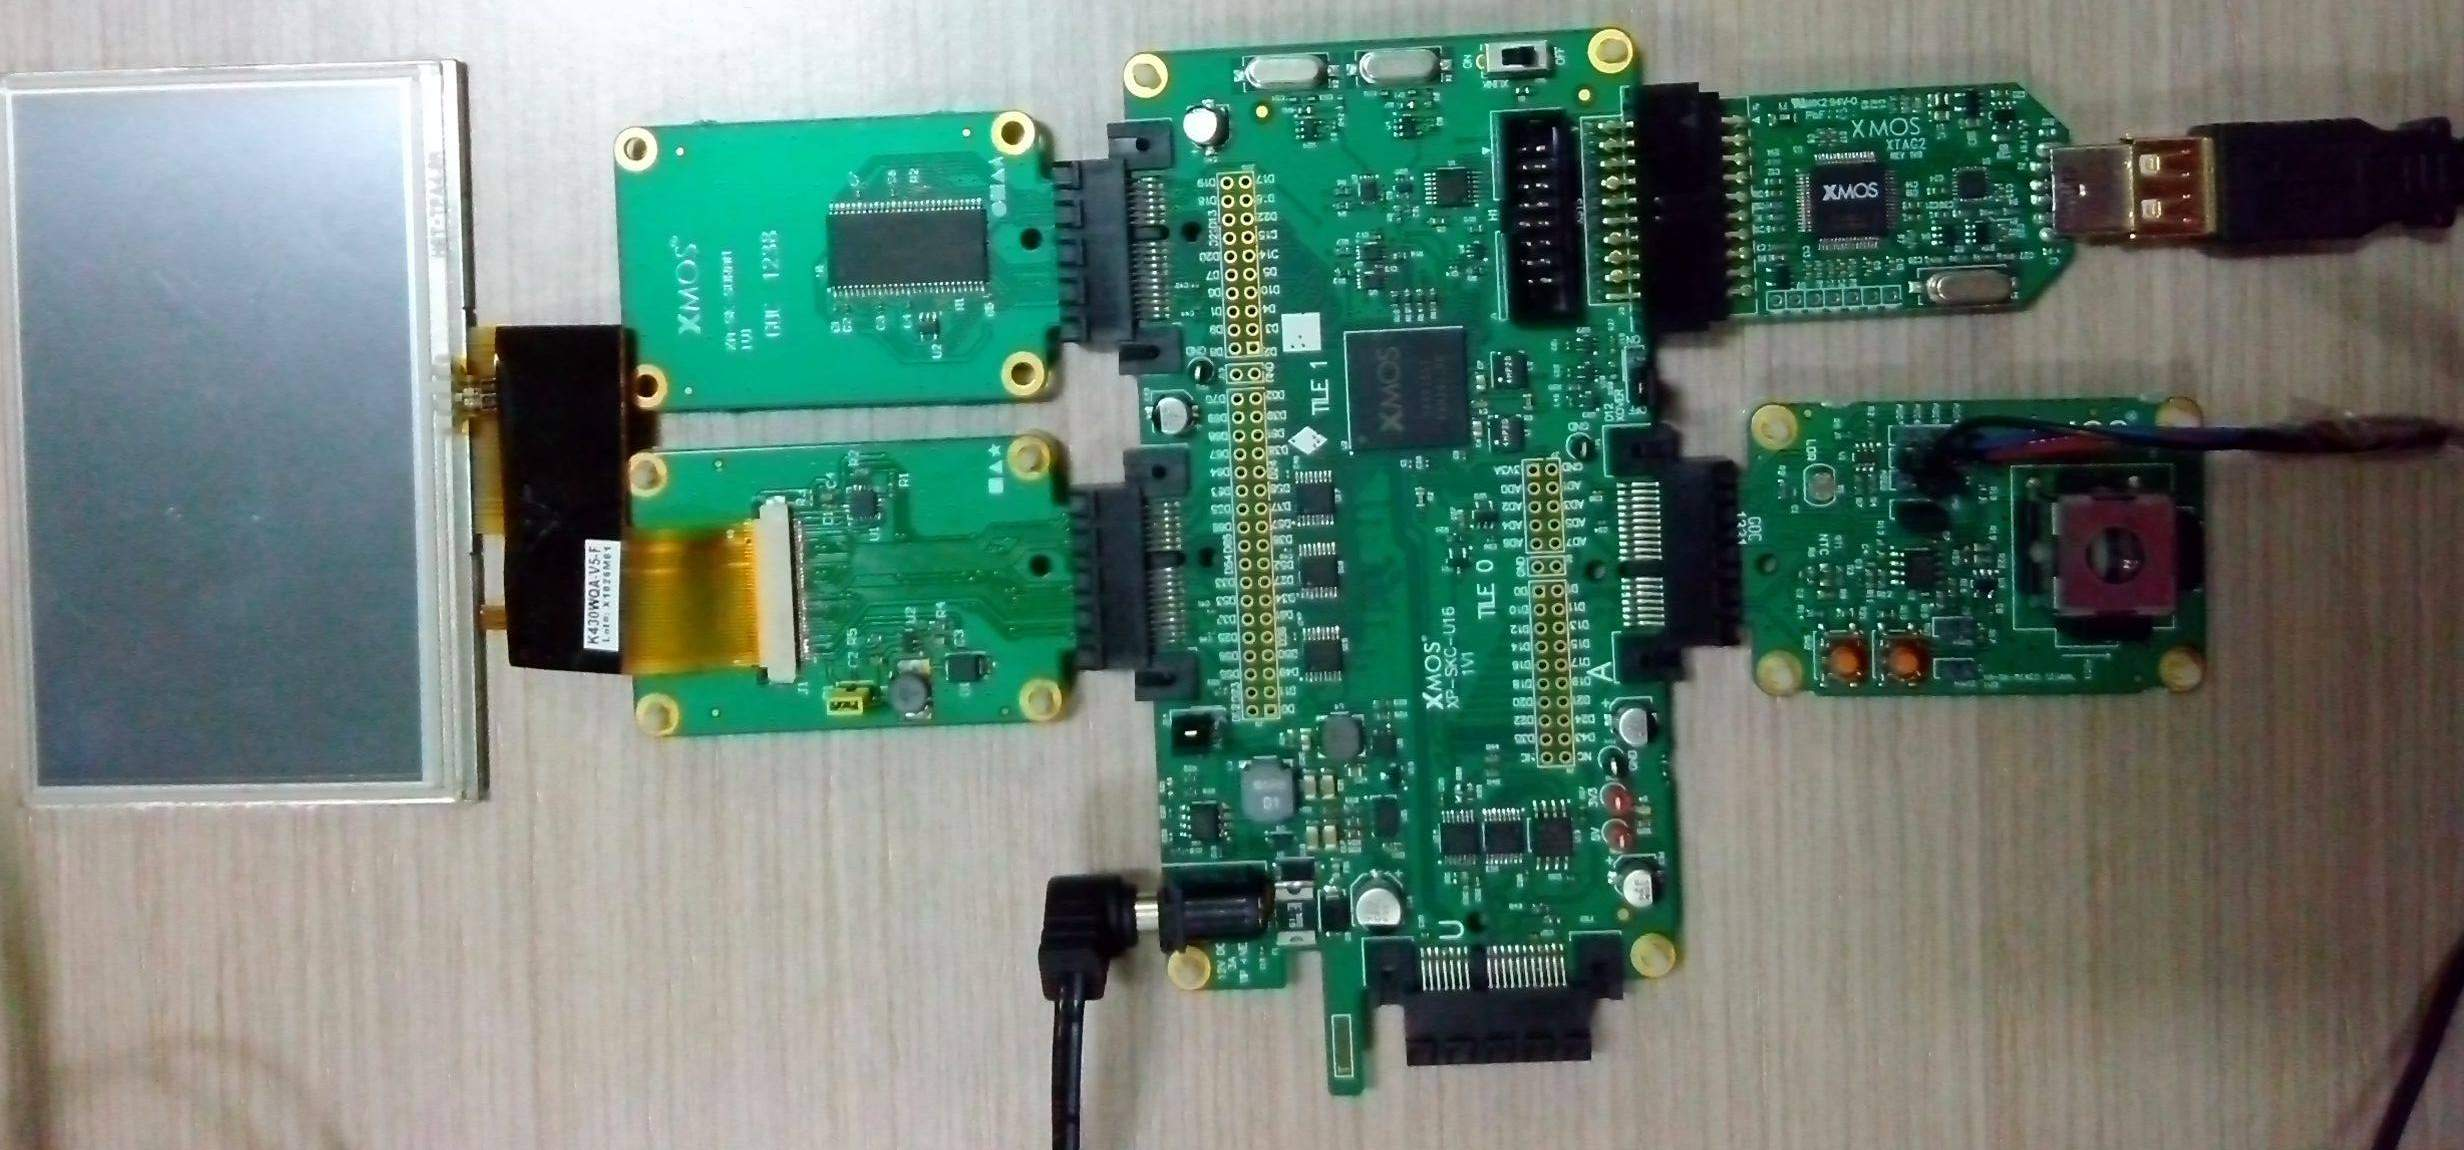
\includegraphics[width=10cm]{hardware_setup.jpg}
\end{sidecaption}\end{figure} \DocumentFooterFix



% NON-FULLWIDTH SECTION
\section{Import and Build the Application}
\label{quickstart:import-and-build-the-application}\begin{enumerate}
\item   Open xTIMEcomposer and check that it is operating in online mode. Open the edit perspective (Window-\textgreater{}Open Perspective-\textgreater{}XMOS Edit).

\item   Locate the \verb`Display Spectrum from ADC Demo` item in the xSOFTip pane on the bottom left of the window and drag it into the Project Explorer window in the xTIMEcomposer. This will also cause the modules on which this application depends to be imported as well.

\item   Include \verb`#define LCD_USE_32_BIT_DATA_PORT 1` in \verb`lcd.xc` located in \verb`module_lcd`.

\item   Click on the \verb`app_display_spectrum_from_adc` item in the Explorer pane then click on the build icon (hammer) in xTIMEcomposer. Check the console window to verify that the application has built successfully.

\item   There will be quite a number of warnings that \verb`bidirectional buffered port not supported in hardware`. These can be safely ignored for this component.

\end{enumerate}



For help in using xTIMEcomposer, try the xTIMEcomposer tutorial, which you can find by selecting Help-\textgreater{}Tutorials from the xTIMEcomposer menu.


Note that the Developer Column in the xTIMEcomposer on the right hand side of your screen provides information on the xSOFTip components you are using.



% NON-FULLWIDTH SECTION
\section{Run the Application}
\label{quickstart:run-the-application}

Now that the application has been compiled, the next step is to run it on the sliceKIT Core Board using the tools to load the application over JTAG (via the xTAG-2) into the xCORE multicore microcontroller.
\begin{enumerate}
\item   Select \verb`app_display_spectrum_from_adc` project from the Project Explorer.

\item   Click on the \verb`Run` icon (the white arrow in the green circle).

\item   At the \verb`Select Device` dialog select \verb`XMOS xTAG-2 connect to L1[0..1]` and click \verb`OK`.

\item   Play an audio in the PC or mobile. A test audio file containing a sine sweep from 20 to 20kHz is available in \verb`app_display_spectrum_from_adc/test_data`.

\item   The spectra of segments of mixed signal of two audio channels are displayed on LCD.

\item   Try changing the volume of the audio input and notice the change in the height of spectral components.

\end{enumerate}




% NON-FULLWIDTH SECTION
\section{Next Steps}
\label{quickstart:next-steps}

Various parameters defined in \verb`app_display_spectrum_from_adc.xc` are listed below. These can be adjusted if necessary.
\begin{enumerate}
\item   \verb`SAMP_FREQ` is the sampling frequency of the analog audio signal.

\item   \verb`FFT_POINTS` give the number of signal samples taken for FFT computation. \verb`FFT_SINE` is defined accordingly.

\item   \verb`LEV_METER_BANDS` give the number of FFT points to be displayed.

\item   \verb`LOG_SPEC` if set to 1 computes log spectrum.

\item   \verb`MAX_FFT` sets the limit for the spectral values to be displayed. Values more than this limit are clipped.

\item   \verb`FFT_FULL_USE` if set puts the FFT computation to full use. If it is 0, then \verb`FFT_UPDATE_RATE` determines the number of times FFT computation is done in a second.

\end{enumerate}



The colors of the level-meter display of spectrum can be changed in \verb`level_meter_conf.h`.




\finish
